% !TeX spellcheck = nl_NL
\documentclass{article}

\begin{document}
	\section{Data-service}
	
	\subsection{De Service}
	Om onze databank aan te spreken gaan we een REST service voorzien waar we enkele simplistische methodes toekennen die het mogelijk maken om: de gewijzigde data periodiek op te halen aan de hand van een datum die fungeert als ondergrens en een endpoint waar we \'e\'en element kunnen ophalen aan de hand van een ID. Dit maakt het mogelijk om periodiek de gewijzigde modellen uit onze databank op te halen en naar AEM te versturen. Of deze manier van werken haalbaar is voor al onze modellen gaan we later uitmaken. Voor producten voorzien we een extra endpoint om deze aan de hand van een categorie op te halen. 
	\par
	We gebruiken hiervoor een Java Spring-boot service omdat deze makkelijk in opzet zijn, gezien het een REST service is kan hier perfect voor een andere programmeertaal gekozen worden. Onze configuratie doen we via een application.yml bestand, deze wordt automatisch door de laatste versie van Spring-boot ondersteund. We voorzien ook de docker-maven-plugin om het onszelf iets makkelijker te maken. We configureren deze zoals Figuur \ref{fig:docker-plugin}. De configuratie die we meegeven is redelijk transparant, imageName duidt aan hoe we onze docker images gaan noemen, een samenstelling van de artifact naam en versie zorgt ervoor dat elke versie van onze service een unieke imageName krijgt. Moest er de nood zijn om een vorige versie terug te zetten, kan dit in een handomdraai. De dockerDirectory duidt waar we onze image willen aanmaken, de properties onder resources vertelt Docker wat er in de image moet worden opgenomen. Als Docker correct ge\"installeerd is, kunnen we het commando 'mvn clean package docker:build' uitvoeren om onze image te bouwen.
	
	\begin{figure}[h!]
		\centering
  		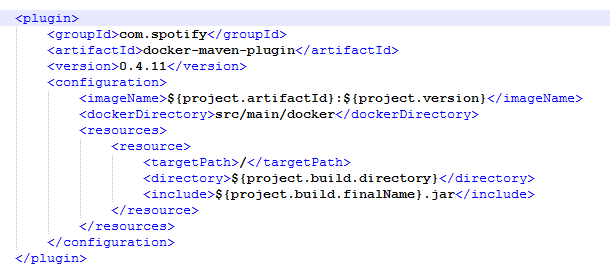
\includegraphics[width=\linewidth]{images/maven-plugin.PNG}
  		\caption{Maven Docker Plugin.}
  		\label{fig:docker-plugin}
	\end{figure}

\par
Om te connecteren met onze Cassandra cluster maken we gebruik van de Datastax java-driver. Datastax is een bedrijf dat een commerciële versie van Apache Cassandra aanbiedt alsook support voorziet. Hun Java-driver is open-source en dus gratis te gebruiken, deze driver biedt een betere ondersteuning voor het gebruik van UDTs tegenover de JPA-implementatie voor Cassandra. Om deze driver te gebruiken moeten we onze klassen die overeenstemmen met een tabel in onze databank annoteren met ‘@Table’. De velden in deze klassen krijgen nog de annotatie ‘@Column’ en ‘@PartitionKey’ als het gaat om een primary key kolom. Voor de types van onze databank voorzien we ook klassen voor die we annoteren met ‘@Field’. De velden hier annoteren we met ‘@Field’. Eenmaal we onze tabellen hebben vertaald naar overeenstemmende klassen volstaat het om een sessie met onze cluster aan te maken, bij het aanmaken hiervan volstaat het om het IP-adres van \'e\'en node te voorzien, de driver zal dan via discovery de locatie van de overige nodes vinden en zo fouttolerantie te waarborgen. Het is toch aan te raden om meerdere IP-adressen mee te geven zodat wanneer er een node niet beschikbaar is tijdens het aangaan van de sessie, deze kan terugvallen op een andere node. Verder voorzien we per model een REST controller met de methoden die we reeds besproken hebben.
\par
	\subsection{Docker}
	De volgende stap in ons process is een manier zoeken om onze service in de cloud te draaien. Het is aanvaardbaar om tijdens de ontwikkeling onze service lokaal te draaien maar als we een volwaardig platform willen cre\"eren moet ook dit onderdeel remote draaien.
	\par
	\begin{wrapfigure}{r}{0.5\textwidth}
  	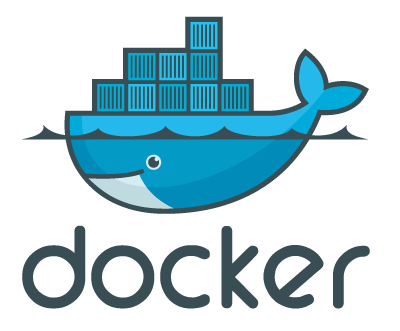
\includegraphics[width=0.4\textwidth]{images/docker-logo.PNG}
	\end{wrapfigure}
	
	Docker is een open-source project dat dit process voor ons zal versimpelen. 
    Vroeger moest er heel wat tijd (en bijgevolg ook budget) gespendeerd worden aan het werkende krijgen van services op verschillende machines. 
    Dit komt omdat niet alle machine hetzelfde geconfigureerd zijn en niet elke machine ondersteunt alles even goed. 
    Docker lost dit probleem op door maar \'e\'en vereiste te hebben, dat de machines de Docker service hebben draaien. Oorspronkelijk ondersteunde enkel Linux systemen deze service native maar ondertussen zijn ook Windows en Mac mee op de kar gesprongen. Om deze lokaal te trainen, voor testing doeleinden, kan men naar de docker website gaan en de gewenste versie downloaden. De tutorials die je daar kan vinden leggen perfect uit hoe je ermee aan de slag kan. Natuurlijk gaan we, na een korte uitlichting, onze Docker remote gaan draaien.
	\par
	Wie Docker zegt, zegt containers. Om onafhankelijk van de host een applicatie te kunnen draaien, steekt Docker deze, en al het nodige (environment, tools, libraries,settings,...), in een container. Docker bundelt al het nodige samen en maakt er een exporteerbare image van. Deze image kunnen we dan eender waar draaien zonder ons zorgen te moeten maken om infrastructurele verschillen. Dit wil zeggen dat wanneer een image succesvol in een trainingsomgeving draait, deze zonder vrees overgezet kan worden naar een productie omgeving.
	\par
	Een ander voordeel van het containersysteem is dat men elke container, tijdens het opstarten, specifieke parameters kan meegeven met betrekking tot de resources die deze ter beschikking krijgt. Als men enkele zwaardere services heeft, kan met de container hiervan meer RAM toekennen om aan de behoefte te voldoen. Het is perfect mogelijk om meerdere containers op \'e\'en machine of verdeelt over meerdere machines te draaien wat de schaalbaarheid en beschikbaarheid waarborgt. Zelfs een release hoeft geen downtime meer te betekenen, de containers kunnen \'e\'en voor \'e\'en vervangen worden met een nieuwere versie.
	\par
	Buiten de configuratie met betrekking tot de resources kan men ook omgevingsvariabelen meegeven (hoe dit mogelijk is zien we dadelijk). Dit heeft als voordeel dat we dezelfde container kunnen gebruiken voor onze trainings -en productieomgeving door ander variabelen, zoals de databaselocatie en credentials, urls van andere services, enz., mee te geven tijdens het starten van onze containers.
	\subsection{AWS en Docker}
	Nu wordt het tijd dat we onze services in de cloud gaan draaien. Hiervoor zijn enkele stappen nodig beginnend bij de installatie van de nodige software op onze ontwikkelingsmachine. De eerste installatie is die van de AWS Command Line Interface (of kortweg AWS CLI), gelukkig voor ons heeft Amazon hier een uitstekende handleiding\footnote{http://docs.aws.amazon.com/cli/latest/userguide/installing.html}
	voor. Het is belangrijk niet te vergeten om na de installatie deze ook te configureren\footnote{http://docs.aws.amazon.com/cli/latest/userguide/cli-chap-getting-started.html}.
	\par
	Het tweede wat we nodig zullen hebben is Docker op onze ontwikkelingsmachine, niet omdat we onze containers hier gaan draaien maar omdat we deze hier gaan bouwen. Voor diegene zonder ervaring met Docker raad ik deze manier aan om een beter begrip te krijgen van hoe dit in zijn werk gaat. De ervaren lezer mag natuurlijk zijn images op zijn gekozen manier bouwen. Om Docker te installeren kan de Linux-gebruiker zijn shell gebruiken, Mac en Windows hebben minder geluk en zullen een installer\footnote{https://docs.docker.com/engine/installation/} moeten gebruiken.
	\par
	Eenmaal onze ontwikkelingsmachine klaar is, keren we terug naar AWS om een ECS-cluster (EC2 Container Service) op te zetten, hierin gaan we onze containers laten draaien. Een cluster kan men zien als een logische groepering van machines, wanneer we dezelfde image meermaals deployen zullen de benodigde containers automatisch verdeeld worden over de machines in onze cluster.
	\par
	Voor we aan onze cluster beginnen maken we snel 2 IAM rollen aan, \'e\'en rol voor onze machines en \'e\'en rol voor de service die we op onze cluster zullen starten. De rol voor de machines geven we een logische naam: ecs-instance-role en geven we de permissie AmazonEC2ContainerServiceforEC2Role {Geeft de machine schrijfrechten op CloudWatch en ECS, leesrechten op ECR}. De rol voor de service noemen we ecs-service-role en geven we de de permissie AmazonEC2ContainerServiceRole (schrijf -en leesrechten op EC2 en ELB). 
	\par	
	 Een ECS cluster opzetten is geen werk, even navigeren naar het scherm, kiezen om een nieuwe te maken, we geven deze een naam (bv. tst-ecs-cluster) en voor nu selecteren we de optie 'Create an empty cluster'. Wanneer we deze cluster aanmaken dan zien we deze verschijnen maar zonder machines in, deze toevoegen is een volgende stap.
	\par
	Vervolgens maken we een Launch configuration aan, dit zal beschrijven hoe onze machines opgestart moeten worden. De configuratie heeft als voordeel dat we dit maar eenmaal moeten doen en dat alle machines binnen onze cluster met dezelfde configuratie opstarten. Dit is grotendeels gelijk aan het maken van een machine, let wel op dat je als AMI\footnote{Amazon Machine Image} de Amazon ECS-optimized\footnote{te vinden onder AWS Marketplace} kiest. Dit zal onze machines automatisch van Docker voorzien en deze starten wanneer de machine boot. Ken de ecs-instance-rol toe aan onze machines bij de stap Configure details. In deze stap voegen we ook een script toe onder User data (Advanced Details). Hier schrijven we het script als gezien in Figuur \ref{fig:ecs-script}. Dit zorgt ervoor dat de machines die met deze configuratie starten aan onze cluster worden toegevoegd.
	\begin{figure}[h!]
		\centering
  		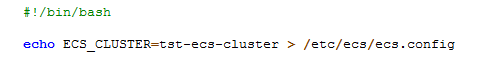
\includegraphics[width=0.5\textwidth]{images/ecs-script.PNG}
  		\caption{ECS bootup script.}
  		\label{fig:ecs-script}
	\end{figure}
	\par
	Nu we een Launch configuration hebben kunnen we deze gebruiken om effectief machines aan te maken. Dit doen we door een Auto Scaling Group aan te maken via de EC2 module. Tijdens het opzetten van deze groep kiezen we de Launch configuration die we juist hebben aangemaakt. We geven de groep een naam en hoeveel machines we willen bij de opstart ervan alsook een subnet. Dit subnet kan gebruikt worden om strengere security filters in te stellen door enkel machines binnen dit subnet met elkaar te laten communiceren. Men zou dan via routing kunnen werken om een bepaald deel van de endpoints publiek toegankelijk te maken. In dit project gaan we hier niet verder op in. Onder Scaling Policies kunnen we beschrijven onder welke voorwaarden er meer machines moeten worden bijgezet, bijvoorbeeld als het CPU verbruik van onze cluster gedurende 5 minuten boven de 80\% is. Omgedraaid kunnen we ook instellen wanneer er machines verwijderd mogen worden buiten de piekuren. Als alles goed verlopen is zien we na creatie een aantal machines, gelijk aan het gekozen aantal, opstarten onder ons EC2 Instances scherm. Deze machines zouden, dankzij het ecs-script, ook te zien zijn als we bij onze ECS-cluster gaan kijken onder Instances.
	\par
	Nu rest ons enkel nog het toevoegen van een loadbalancer en we zijn klaar om onze Docker containers te bouwen en te deployen naar onze nieuwe cluster. Een loadbalancer fungeert als gateway naar onze machines, inkomende requests op onze loadbalancer worden verdeeld en doorgestuurd naar de machines die de balancer als gezond beschouwt. Om de gezondheid van een machine te controleren doet deze periodiek een request naar de machines, zolang de machines met een status 200 antwoorden beschouwt de balancer ze als gezond. Hoe frequent en hoe vaak een antwoord positief of negatief moet zijn om de status van de machine te veranderen, kan ingesteld worden. Ook de snelheid waarmee de machine moet antwoorden kan geconfigureerd worden, standaard is dit 5 seconden maar als je met gratis micro machines werkt verhoog je dit best. De netwerk capaciteiten van deze machines zijn beperkt waardoor de limiet van 5 seconden overschreven kan worden. Indien dit gebeurt, haalt de balancer deze machines uit rotatie.
	\par
	Het volgende deel van het plan is bouwen van een image, via de maven plugin, en deze uploaden naar onze EC2 Container Repository. Vervolgens kunnen we een nieuwe service defini\"eren voor onze ECS cluster, hiervoor kiezen we als task definition onze docker image. Op het einde van deze stap kunnen we, via de loadbalancer, onze services callen.
\end{document}

